\chapter{Dynaaminen ohjelmointi}

Dynaaminen ohjelmointi on algoritmisuunnittelun tekniikka,
jota voi käyttää kahdenlaisissa tilanteissa:

\begin{itemize}
\item \textbf{Optimiratkaisun etsiminen}: Haluamme etsiä ratkaisun,
joka on jollakin tavalla suurin tai pienin.
\item \textbf{Ratkaisumäärän laskeminen}: Haluamme laskea,
montako erilaista ratkaisua on olemassa.
\end{itemize}

Ideana on muotoilla laskentatehtävä
rekursiivisesti niin, että voimme ratkaista tehtävän
ratkaisemalla ensin osatehtävinä saman tehtävän pienempiä tapauksia.
Aina kun olemme ratkaisseet tietyn osatehtävän,
kirjaamme sen ratkaisun muistiin, minkä ansiosta
pystymme hakemaan ratkaisun tehokkaasti uudestaan,
kun tarvitsemme sitä myöhemmin.

Tässä luvussa tutustumme ensin dynaamisen ohjelmoinnin perusteisiin
käyttäen esimerkkinä tehtävää, jossa haluamme laskea,
monellako tavalla voimme rakentaa tornin palikoista.
Tämän jälkeen käymme läpi joukon muita tehtäviä, jotka esittelevät
dynaamisen ohjelmoinnin mahdollisuuksia.

\section{Perustekniikat}

Aloitamme dynaamiseen ohjelmointiin tutustumisen
seuraavasta tehtävästä:
meillä on palikoita, joiden korkeudet ovat 1, 2 ja 3,
ja haluamme rakentaa niistä tornin, jonka korkeus on $n$.
Jokaista palikkatyyppiä on saatavilla rajattomasti.
Monellako tavalla voimme rakentaa tornin?

\begin{figure}
\center
\begin{tikzpicture}[scale=0.7]
\newcommand\palikka[3]{
\draw (2*#1,#2) rectangle (2*#1+1,#2+#3);
}
\palikka{0}{0}{1} \palikka{0}{1}{1} \palikka{0}{2}{1} \palikka{0}{3}{1}
\palikka{1}{0}{1} \palikka{1}{1}{1} \palikka{1}{2}{2}
\palikka{2}{0}{1} \palikka{2}{1}{2} \palikka{2}{3}{1}
\palikka{3}{0}{2} \palikka{3}{2}{1} \palikka{3}{3}{1}
\palikka{4}{0}{2} \palikka{4}{2}{2}
\palikka{5}{0}{1} \palikka{5}{1}{3}
\palikka{6}{0}{3} \palikka{6}{3}{1}
\end{tikzpicture}
\caption{Voimme rakentaa korkeuden 4 tornin 7 tavalla palikoista,
joiden korkeudet ovat 1, 2 ja 3.}
\label{fig:dyntor}
\end{figure}

Kuva \ref{fig:dyntor} näyttää esimerkin, jossa $n=4$.
Tässä esimerkissä meillä on 7 tapaa rakentaa torni palikoista.
Voimme luonnehtia torneja myös summina luvuista 1, 2 ja 3.
Tässä tapauksessa vasen torni vastaa summaa $1+1+1+1$,
seuraava torni vastaa summaa $1+1+2$, jne.

Jos $n$ on pieni, voimme laskea tornien määrän helposti
käymällä läpi kaikki tavat, mutta tornien määrä kasvaa
nopeasti emmekä voi käyttää raakaa voimaa suuremmilla
$n$:n arvoilla.
Seuraavaksi ratkaisemmekin ongelman tehokkaasti
dynaamisen ohjelmoinnin avulla.

\subsection{Rekursiivinen esitys}

Jotta voimme käyttää dynaamista ohjelmointia,
meidän täytyy esittää ongelma rekursiivisesti
niin, että saamme laskettua ongelman ratkaisun
käyttäen osaongelmina pienempiä vastaavia ongelmia.

Tässä tehtävässä meidän on luontevaa määritellä rekursiivinen
funktio $\texttt{tornit}(n)$: monellako tavalla voimme
rakentaa tornin, jonka korkeus on $n$?
Esimerkiksi $\texttt{tornit}(4)=7$, koska tiedämme
esimerkkimme ansiosta,
että voimme rakentaa korkeuden 4 tornin 7 tavalla.

Funktion pienten arvojen laskeminen on helppoa.
Ensinnäkin $\texttt{tornit}(0)=1$, koska voimme
muodostaa tyhjän tornin yhdellä tavalla:
siinä ei ole mitään palikoita.
Sitten $\texttt{tornit}(1)=1$, koska ainoa mahdollisuus
on valita korkeuden 1 palikka,
ja $\texttt{tornit}(2)=2$, koska voimme joko valita
kaksi korkeuden 1 palikkaa tai yhden korkeuden 2 palikan.

\begin{figure}
\center
\begin{tikzpicture}[scale=0.7]
\draw (0,0) rectangle (1,1);
\draw[dashed] (0,1) rectangle (1,4);
\draw (4,0) rectangle (5,2);
\draw[dashed] (4,2) rectangle (5,4);
\draw (8,0) rectangle (9,3);
\draw[dashed] (8,3) rectangle (9,4);
\draw [decorate,decoration={brace,amplitude=4pt},xshift=0.2cm] (1,4) -- (1,1) node [midway,right,xshift=.1cm] {$n-1$};
\draw [decorate,decoration={brace,amplitude=4pt},xshift=0.2cm] (5,4) -- (5,2) node [midway,right,xshift=.1cm] {$n-2$};
\draw [decorate,decoration={brace,amplitude=4pt},xshift=0.2cm] (9,4) -- (9,3) node [midway,right,xshift=.1cm] {$n-3$};
\end{tikzpicture}
\caption{Rekursiivinen idea: kun alamme rakentaa tornia, voimme laittaa pohjalle
korkeuden 1, 2 tai 3 palikan.}
\label{fig:dynrek}
\end{figure}


Kuinka voisimme sitten laskea funktion arvon yleisessä tapauksessa,
kun tornin korkeus on $n$?
Tässä voimme miettiä, kuinka tornin rakentaminen alkaa.
Meillä on kolme mahdollisuutta: voimme laittaa ensin palikan
korkeutta 1, 2 tai 3.
Jos valitsemme korkeuden 1 palikan, meidän täytyy rakentaa
sen päälle korkeuden $n-1$ torni.
Vastaavasti jos valitsemme korkeuden 2 tai 3 palikan,
meidän täytyy rakentaa sen päälle torni,
jonka korkeus on $n-2$ tai $n-3$.
Kuva \ref{fig:dynrek} havainnollistaa tämän idean.

Niinpä voimme laskea tornien määrän rekursiivisesti kaavalla
\[
\texttt{tornit}(n) = \texttt{tornit}(n-3)+\texttt{tornit}(n-2)+\texttt{tornit}(n-1),
\]
kun $n \ge 3$.
Esimerkiksi voimme laskea
\[
\texttt{tornit}(3) = \texttt{tornit}(0)+\texttt{tornit}(1)+\texttt{tornit}(2)=4
\]
ja
\[
\texttt{tornit}(4) = \texttt{tornit}(1)+\texttt{tornit}(2)+\texttt{tornit}(3)=7,
\]
jolloin olemme saaneet laskettua esimerkkitapaustamme vastaavasti,
että voimme rakentaa korkeuden 4 tornin 7 tavalla.

\begin{table}
\center
\begin{tabular}{rrr}
korkeus $n$ & $\texttt{tornit}(n)$ \\
\hline
0 & 1 \\
1 & 1 \\
2 & 2 \\
3 & 4 \\
4 & 7 \\
5 & 13 \\
6 & 24 \\
7 & 44 \\
8 & 81 \\
9 & 149 \\
\end{tabular}
\caption{Tornien määrät, kun korkeus $n$ on $0,1,\dots,9$.}
\label{tab:dyntor}
\end{table}

Taulukko \ref{tab:dyntor} näyttää yhteenvedon funktion
$\texttt{tornit}(n)$ arvoista, kun $n=0,1,\dots,9$.
Kuten taulukosta voi huomata, funktion arvo kasvaa nopeasti:
se lähes kaksinkertaistuu joka askeleella.
Kun $n$ on suuri,
meillä onkin valtavasti mahdollisuuksia tornin rakentamiseen.

\subsection{Tehokas toteutus}

Nyt kun olemme saaneet aikaan rekursiivisen funktion,
voimme toteuttaa sen ohjelmoimalla seuraavasti:

\begin{code}
long tornit(int n) {
    if (n == 0) return 1;
    if (n == 1) return 1;
    if (n == 2) return 2;
    return tornit(n-3)+tornit(n-2)+tornit(n-1);
}
\end{code}

Tämä on toimiva ratkaisu, mutta siinä on yksi ongelma:
funktion arvon laskeminen vie kauan aikaa, jos $n$ on
vähänkin suurempi.
Käytännössä laskenta alkaa hidastua parametrin $n=30$ tienoilla.
Esimerkiksi arvon $\texttt{tornit}(40)$ laskeminen vie aikaa
jo useita minuutteja, ja voimme arvioida, että
arvon $\texttt{tornit}(50)$ laskeminen veisi aikaa noin vuorokauden.

Syynä laskennan hitauteen on, että metodia $\texttt{tornit}$
kutsutaan uudestaan ja uudestaan samoilla parametreilla
ja tornien määrä lasketaan loppujen lopuksi summana
luvuista 1 ja 2 pohjatapauksista.
Niinpä kun tornien määrä on suuri,
laskenta on tuomittu viemään kauan aikaa.
Voimme kuitenkin selviytyä ongelmasta toteuttamalla
laskennan hieman toisella tavalla.

Tässä astuu kuvaan dynaamisen ohjelmoinnin keskeinen idea:
laskemme funktion arvon kullekin parametrille vain kerran
ja tallennamme tulokset taulukkoon myöhempää käyttöä varten.
Tätä varten luomme taulukon $\texttt{tornit}$,
jossa kohtaan $\texttt{tornit}[i]$ tallennetaan funktion
arvo $\texttt{tornit}(i)$.
Kun haluamme laskea korkeuden $n$ tornien määrän,
täytämme taulukon kohdat $0,1,\dots,n$.
Seuraava koodi toteuttaa laskennan:

\begin{code}
long[] tornit = new long[n+1];
tornit[0] = 1;
tornit[1] = 1;
tornit[2] = 2;
for (int i = 3; i <= n; i++) {
    tornit[i] = tornit[i-3]+tornit[i-2]+tornit[i-1];
}
\end{code}

Koodin suorituksen jälkeen taulukon arvo $\texttt{tornit}[n]$
kertoo meille, monellako tavalla voimme rakentaa
korkeuden $n$ tornin.

Tämän toteutuksen etuna on, että se on huomattavasti
nopeampi kuin rekursiivinen metodi.
Koska koodissa on vain yksi for-silmukka, se vie aikaa
vain $O(n)$, eli voimme käsitellä tehokkaasti myös
suuria $n$:n arvoja.
Esimerkiksi voimme nyt laskea salamannopeasti, että
\[
\texttt{tornit}(50) = 10562230626642,
\]
eli meillä on yli 10562 miljardia tapaa rakentaa korkeuden 50 torni.

\section{Esimerkkejä}

Olemme nyt tutustuneet dynaamisen ohjelmoinnin perusideaan,
mutta tämä on vasta alkua sille, mitä kaikkea tekniikan
avulla pystyy tekemään.
Seuraavaksi käymme läpi joukon tehtäviä,
jotka esittelevät lisää dynaamisen ohjelmoinnin mahdollisuuksia.

Jotta voimme käyttää dynaamista ohjelmointia ongelman
ratkaisemiseen, meidän täytyy pystyä muotoilemaan ongelma
rekursiivisesti niin, että voimme tallentaa muistiin
jokaisen osaongelman ratkaisun.
Käytännössä haasteena on keksiä, mikä on hyvä rekursiivinen
muotoilu ongelmalle.

\subsection{Pisin nouseva alijono}

Ensimmäinen ongelmamme on selvittää, kuinka pitkä on
$n$ alkiota sisältävän taulukon \emph{pisin nouseva alijono}.
Tämä tarkoittaa, että meidän tulee valita taulukosta
mahdollisimman pitkä jono alkioita niin,
että seuraava alkio on aina edellistä suurempi.
Kuvassa \ref{fig:pisnou} on esimerkki taulukosta,
jonka pisin nouseva alijono $[2,5,7,8]$ on pituudeltaan 4.

\begin{figure}
\center
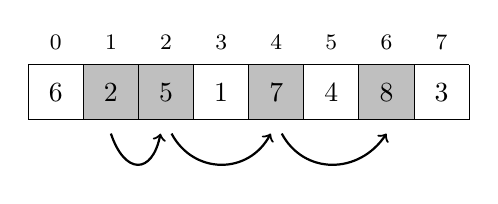
\begin{tikzpicture}[scale=0.7]
\fill[color=lightgray] (1,0) rectangle (2,1);
\fill[color=lightgray] (2,0) rectangle (3,1);
\fill[color=lightgray] (4,0) rectangle (5,1);
\fill[color=lightgray] (6,0) rectangle (7,1);
\draw (0,0) grid (8,1);
\node at (0.5,0.5) {$6$};
\node at (1.5,0.5) {$2$};
\node at (2.5,0.5) {$5$};
\node at (3.5,0.5) {$1$};
\node at (4.5,0.5) {$7$};
\node at (5.5,0.5) {$4$};
\node at (6.5,0.5) {$8$};
\node at (7.5,0.5) {$3$};
\draw[thick,->] (1.5,-0.25) .. controls (1.75,-1.00) and (2.25,-1.00) .. (2.4,-0.25);
\draw[thick,->] (2.6,-0.25) .. controls (3.0,-1.00) and (4.0,-1.00) .. (4.4,-0.25);
\draw[thick,->] (4.6,-0.25) .. controls (5.0,-1.00) and (6.0,-1.00) .. (6.5,-0.25);
\footnotesize
\node at (0.5,1.4) {$0$};
\node at (1.5,1.4) {$1$};
\node at (2.5,1.4) {$2$};
\node at (3.5,1.4) {$3$};
\node at (4.5,1.4) {$4$};
\node at (5.5,1.4) {$5$};
\node at (6.5,1.4) {$6$};
\node at (7.5,1.4) {$7$};
\end{tikzpicture}
\caption{Taulukon pisin nouseva alijono on $[2,5,7,8]$.}
\label{fig:pisnou}
\end{figure}

Voimme lähestyä tehtävää laskemalla jokaiselle taulukon
kohdalle $k=0,1,\dots,n-1$ arvon $\texttt{pisin}(k)$:
kuinka pitkä on pisin nouseva alijono, joka päättyy kohtaan $k$.
Kun olemme laskeneet kaikki nämä arvot, suurin arvoista kertoo meille,
kuinka pitkä on pisin nouseva alijono koko taulukossa.
Esimerkiksi kuvan \ref{fig:pisnou} taulukossa $\texttt{pisin}(6)=4$,
koska kohtaan $6$ päättyvä pisin nouseva alijono on pituudeltaan $4$.

Millainen on sitten pisin kohtaan $k$ päättyvä alijono?
Yksi mahdollisuus on, että alijonossa on vain kohdan $k$ alkio,
jolloin $\texttt{pisin}(k)=1$.
Muussa tapauksessa alijono muodostuu niin,
että siinä on ensin kohtaan $x$ päättyvä
pisin nouseva alijono, missä $x<k$, ja sitten vielä kohdan $k$ alkio.
Tämä edellyttää, että kohdan $x$ alkio on pienempi
kuin kohdan $k$ alkio.
Tuloksena olevan alijonon pituus on $\texttt{pituus}(x)+1$.
Voimmekin käydä läpi kaikki mahdolliset tavat valita kohta $x$
ja ottaa niistä parhaan vaihtoehdon.

Seuraava koodi laskee jokaiselle $k=0,1,\dots,n-1$
pisimmän kohtaan $k$ päättyvän alijonon pituuden yllä kuvattua
ideaa käyttäen.
Koodi olettaa, että taulukon sisältö on taulukossa \texttt{taulu},
ja se muodostaa taulukon \texttt{pisin}, jossa on pisimpien
alijonojen pituudet.

\begin{code}
for (int k = 0; k < n; k++) {
    pisin[k] = 1;
    for (int x = 0; x < k; x++) {
        if (taulu[x] < taulu[k] && pisin[x]+1 > pisin[k]) {
            pisin[k] = pisin[x]+1;
        }
    }
}
\end{code}

Koodin suorituksen jälkeen pisimmän nousevan alijonon pituus on
siis suurin taulukon \texttt{pisin} arvoista.
Tämä algoritmi vie aikaa $O(n^2)$, koska siinä on kaksi
sisäkkäistä silmukkaa.

Mitä jos haluaisimme selvittää pisimmän nousevan alijonon
pituuden lisäksi, mistä alkioista se muodostuu?
Tämä onnistuu laajentamalla hieman koodia.
Ideana on rakentaa taulukko \texttt{aiempi},
joka kertoo jokaisessa kohdassa, missä on tähän kohtaan
päättyvän pisimmän alijonon edellinen alkio.
Voimme muodostaa taulukon seuraavasti:

\begin{code}
for (int k = 0; k < n; k++) {
    pisin[k] = 1;
    aiempi[k] = -1;
    for (int x = 0; x < k; x++) {
        if (taulu[x] < taulu[k] && pisin[x]+1 > pisin[k]) {
            pisin[k] = pisin[x]+1;
            aiempi[k] = x;
        }
    }
}
\end{code}

Tämän jälkeen jokaisessa kohdassa $k$ arvo $\texttt{aiempi}[k]$
kertoo pisimmän alijonon edellisen alkion kohdan.
Kuitenkin jos alijonon pituus on 1, taulukossa on arvo $-1$.
Voimme selvittää kohtaan $k$ päättyvän alijonon alkiot
käänteisesti seuraavasti:

\begin{code}
while (k != -1) {
    print(taulu[k]);
    k = aiempi[k];
}
\end{code}

Voimme käyttää vastaavaa tekniikkaa
dynaamisessa ohjelmoinnissa aina, kun haluamme
selvittää, miten voimme muodostaa parhaan ratkaisun.

\subsection{Reitti ruudukossa}

Olemme $n \times n$ -ruudukon vasemmassa yläkulmassa ja haluamme
päästä oikeaan alakulmaan.
Jokaisella vuorolla voimme siirtyä ruudun alaspäin tai oikealle.
Kuitenkin joissakin ruuduissa on este, emmekä voi kulkea sellaisen
ruudun kautta.
Montako mahdollista reittiä on olemassa?

\begin{figure}
\center
\begin{tikzpicture}[scale=0.7]
\newcommand\ruudukko{
\fill[color=gray] (1,1) rectangle (2,2);
\fill[color=gray] (1,3) rectangle (2,4);
\fill[color=gray] (3,2) rectangle (4,3);
\draw (0,0) grid (4,4);
}
\begin{scope}
\ruudukko
\draw[thick,->,red,line width=2pt] (0.5,3.5) -- (0.5,0.5) -- (3.5,0.5);
\end{scope}
\begin{scope}[xshift=5.5cm]
\ruudukko
\draw[thick,->,red,line width=2pt] (0.5,3.5) -- (0.5,2.5) -- (2.5,2.5) -- (2.5,0.5) -- (3.5,0.5);
\end{scope}
\begin{scope}[xshift=11cm]
\ruudukko
\draw[thick,->,red,line width=2pt] (0.5,3.5) -- (0.5,2.5) -- (2.5,2.5) -- (2.5,1.5) -- (3.5,1.5) -- (3.5,0.5);
\end{scope}
\end{tikzpicture}
\caption{Mahdolliset reitit vasemmasta yläkulmasta oikeaan alakulmaan.}
\label{fig:reiruu}
\end{figure}

Kuvassa \ref{fig:reiruu} on esimerkkitilanne, jossa ruudukon koko on $4 \times 4$.
Tässä tapauksessa meillä on kolme mahdollisuutta, kuinka voimme liikkua
vasemmasta yläkulmasta oikeaan alakulmaan.

Tässä tehtävässä ratkaisun tila on \emph{kaksiulotteinen},
koska olemme reitin joka vaiheessa tietyn rivin tietyllä sarakkeella.
Niinpä määritte\-lemme rekursiivisen funktion, jolla on kaksi
parametria: $\texttt{reitit}(y,x)$ kertoo, montako reittiä on
vasemmasta yläkulmasta ruutuun $(y,x)$.
Tätä funktiota käyttäen $\texttt{reitit}(n,n)$ antaa meille
vastauksen tehtävään.

Olennainen havainto on, että jokaisessa ruudussa meillä on kaksi
mahdollisuutta, kuinka reitti voi tulla ruutuun,
koska voimme tulla joko ylhäältä tai vasemmalta.
Kun haluamme laskea reittien määrää, laskemme yhteen ylhäältä
ja vasemmalta tulevat reitit.
Rajoituksena jos ruudussa on este, siihen tulevien reittien
määrä on aina nolla.

Voimme toteuttaa dynaamisen ohjelmoinnin seuraavasti:

\begin{code}
reitit[1][1] = 1;
for (int y = 1; y <= n; y++) {
    for (int x = 1; x <= n; x++) {
        if (este[y][x]) continue;
        reitit[y][x] += reitit[y-1][x];
        reitit[y][x] += reitit[y][x-1];
    }
}
\end{code}

Aluksi merkitsemme muistiin, että vasempaan yläkulmaan on yksi reitti,
koska lähdemme liikkeelle siitä.
Tämän jälkeen laskemme reittien määrän kaikkiin muihin ruutuihin.
Jos ruudussa on este, siihen ei tule mitään reittiä,
ja muuten laskemme yhteen ylhäältä ja vasemmalta tulevat reitit.
Tuloksena on koodi, joka vie aikaa $O(n^2)$.

Huomaa, että tässä käytämme taulukon indeksejä $1,2,\dots,n$
ja oletamme, että indekseissä $0$ on arvona nolla.
Tämä on kätevää, koska meidän ei tarvitse tehdä erikoistapauksia
ruudukon yläreunaa ja vasenta reunaa varten.

\subsection{Repunpakkaus}